%%==================================================
%% chapter05.tex for BIT Master Thesis
%%==================================================
\chapter{算法实验和系统测试}
第四章对系统所使用的工具和算法原理进行了介绍,为基于GeoHash的矢量地图渲染添加了功能,设计了基于GeoHash的距离计算优化的方法,并在此基础上设计了基于GeoHash的路径规划算法,同时,基于地理位置区块链的工作设计了区域调度车辆的方法,在这些工作的基础上加入真实场景的业务逻辑,实现了完整的出租车调度系统。本章通过实验对算法的正确性进行了验证,此外还对算法的参数进行对比调节,接着对比了传统区块链环境和地理位置区块链环境所支持的系统的差异,最后在模拟网格地图和真实地图上进行了实验,验证本文所实现的调度系统的实用性。
% 张禹:
% 实验环境
% 调节OHMMM算法边界值(一个流程图,三个数据图)
% 近似算法参数优化,设置容量上限为200(一图一表)
% 直接路况精度
%   差错率:带转向延迟的差错率更低,且不带来计算开销(两图)
%   分析了三种车辆异常行为
% 间接补充的路况精度
%   补充路况能够有效提高路况覆盖率(两图)
% 路况结果分析
%   路况统计比轨迹点统计更平滑(一图)
%   统计道路速度(一图)
%   统计路口转向延迟,和道路速度对比关系,证明正确性(一图)
%   展示矢量地图路况(一图)
% 总结

\section{距离计算优化实验}
这部分工作是对本文提出的距离计算优化的效果进行实验验证。考虑出租车调度系统的规模,本部分探究了距离在20km内的起点和终点GeoHash进行距离计算的运算效果。每组实验进行1000次,取结果的平均值。收集优化前后的距离计算算法结果的响应时间和区块链gas消耗,作为对比优化前后性能的参考,结果如图\ref{fig:betterDistance}和\ref{fig:betterGas}:

\begin{figure}
  \centering
  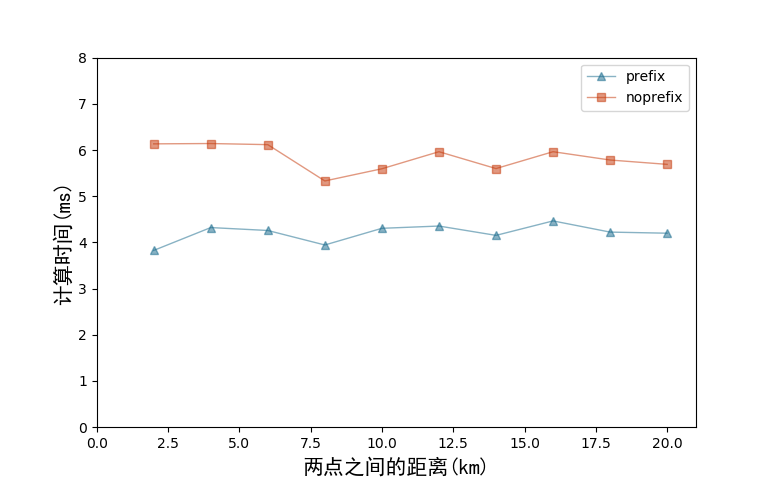
\includegraphics[width=1.0\textwidth]{figures/距离计算优化时间}
  \caption{距离计算优化时间}\label{fig:betterDistance}
\end{figure}

\begin{figure}
  \centering
  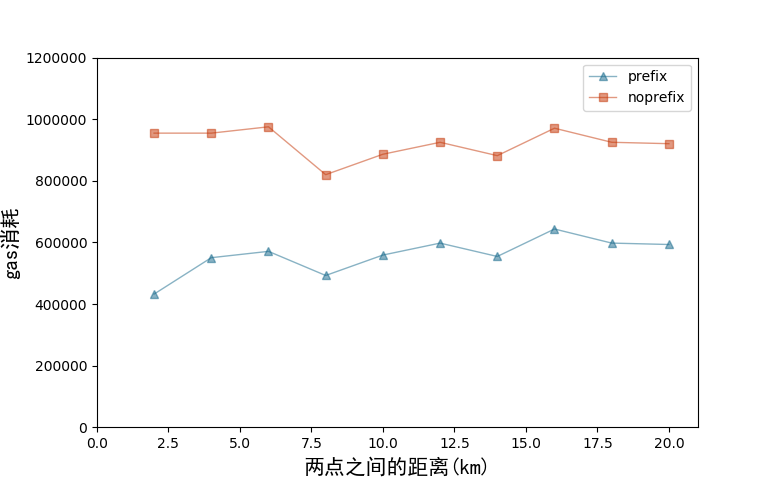
\includegraphics[width=1.0\textwidth]{figures/距离计算优化gas}
  \caption{距离计算优化gas}\label{fig:betterGas}
\end{figure}

由图分析可知,在20km内不同距离的起止点规模下,前缀优化算法在响应时间上对距离计算的性能提升为28$\%$左右,算法优化后的gas消耗也有明显减少,值得注意的是,算法的计算速度与两点之间距离的远近没有明显的相关性。考虑到GeoHash块的大小,4位GeoHash块的南北长约19.54千米,东西长约28.96千米,因此距离在20km的范围内的两个起止点GeoHash通常前3位及以上的字符是相同的,因此进行计算优化后的优化效果比较明显。但考虑到边界情况,位于GeoHash划分边界的20km范围内的两点GeoHash也有前三位的字符不同的时候。

为了探究边界条件下距离优化算法的表现,本文考虑距离20km内的两点,改变两点相同前缀的位数,收集各个位数下距离计算的响应时间和gas消耗,得到算法优化前后两点GeoHash前缀字符相同的位数与算法运行性能的关系如下图\ref{fig:diffBetterTime}和\ref{fig:diffBetterGas}:

\begin{figure}
  \centering
  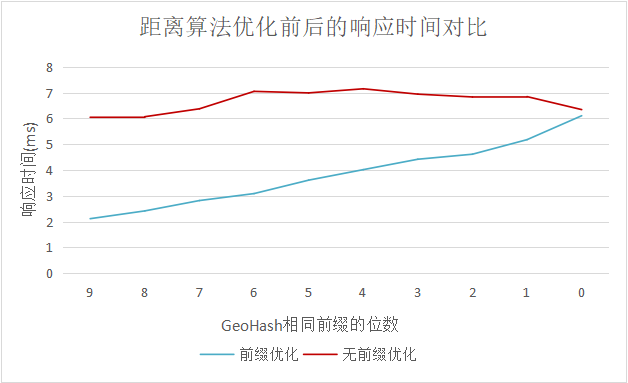
\includegraphics[width=1.0\textwidth]{figures/不同位数优化时间}
  \caption{不同位数优化时间}\label{fig:diffBetterTime}
\end{figure}

\begin{figure}
  \centering
  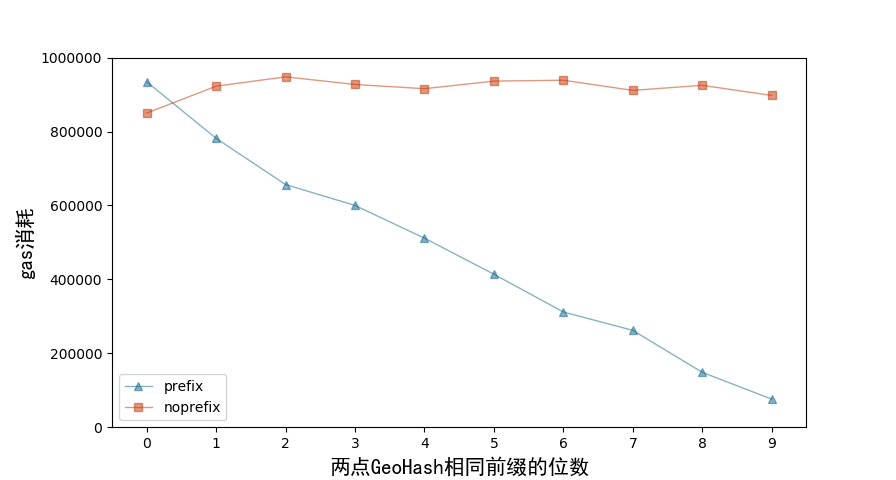
\includegraphics[width=1.0\textwidth]{figures/不同位数优化gas}
  \caption{不同位数优化gas}\label{fig:diffBetterGas}
\end{figure}

由图中结果可知,在考虑两点在GeoHash划分的边界的特殊情况下,这两个点的GeoHash字符串中前缀相同的位数长短,会影响距离计算的速度。相同的前缀越长,距离计算优化后的计算效率提升越明显。
% 算法正确性实验
%   路径规划算法的路径规划结果正确性展示图(一图,或一模拟图一真实图)

\section{路径规划算法参数实验}
本文用上述优化后的GeoHash距离计算得到的真实地理距离作为astar路径规划算法的启发函数结果。

路径规划算法的启发函数的距离计算精度可以通过调节GeoHash的精度来改变,路径规划算法进行计算的精度最高到达10位GeoHash。图中nopre代表没有经过距离计算速度优化且计算精度最高(即基于10位GeoHash的格子大小进行计算)的路径规划算法,pre\_10代表距离计算速度优化后且计算精度最高(基于10位GeoHash)的路径规划算法,pre\_9代表基于9位GeoHash格子大小的精度进行计算的路径规划算法,以此类推,pre\_7代表基于7位GeoHash格子大小的精度进行计算的路径规划算法。

本部分针对不同计算精度下的路径规划算法准确度进行了实验,旨在保证路径规划算法的正确性和结果精度的情况下,提高路径规划算法的计算性能。考虑起止点的直线距离在3km到30km内的规模,在此规模内选取不同距离的起止点,通过实验获取路径规划结果的实际路径长度(平均值)和算法消耗时间(平均值)、区块链的gas消耗量,并做对比,找到在保证路径规划正确性的情况下使其计算效率更高的算法参数,实验结果如图\ref{fig:navRoads}、\ref{fig:navTime}、\ref{fig:navGas}。

\begin{figure}
  \centering
  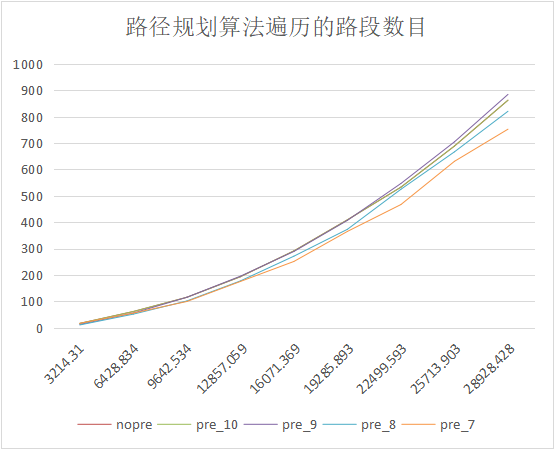
\includegraphics[width=1.0\textwidth]{figures/路径规划路段数目}
  \caption{路径规划路段数目}\label{fig:navRoads}
\end{figure}

\begin{figure}
  \centering
  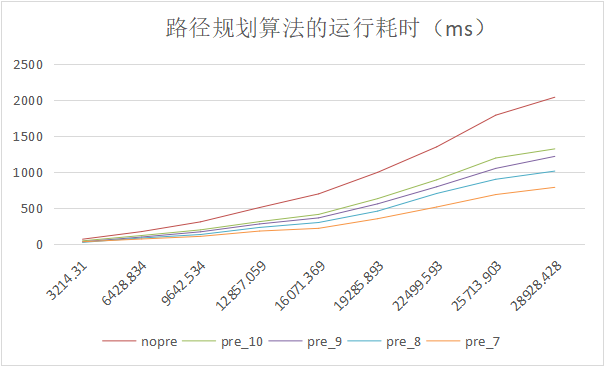
\includegraphics[width=1.0\textwidth]{figures/路径规划耗时}
  \caption{路径规划耗时}\label{fig:navTime}
\end{figure}

\begin{figure}
  \centering
  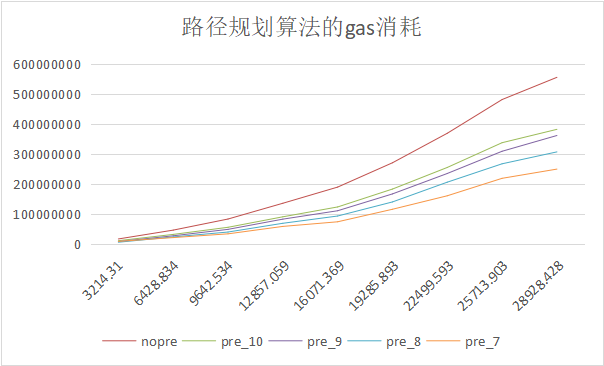
\includegraphics[width=1.0\textwidth]{figures/路径规划gas}
  \caption{路径规划gas}\label{fig:navGas}
\end{figure}

由实验结果可以看出,有无距离计算速度上的优化,对路径规划算法遍历的路段数目影响不明显。同时可以发现,路径规划算法基于的距离计算精度,对路径规划算法遍历路段的数目有一定的影响。值得注意的是,计算距离时基于的GeoHash格子规模扩大后,算法遍历的路段数量略有下降。这是因为格子规模扩大后,启发函数对各路段相距终点的距离计算结果区分度降低,与终点距离相同的中间路段会增多,而算法在遍历到与终点距离相同的各个中间路段时,不会将其重复加入到算法队列中,如此便降低了算法运行时遍历的路段数目。

区块链执行路径规划算法的gas消耗,随着起止点距离的增加会不断增大,主要是因为起止点之间的路段数目增多,算法遍历的路段数增加,导致后台运算的开销增大。实验收集的数据表明,在没有距离计算优化时,GeoHash的路径规划算法消耗的gas数目明显高于优化后的算法,并且随着起止点之间距离的增加,gas消耗的增长趋势也显著增大。

​在GeoHash距离计算的格子规模不同时,可以观察到,随着GeoHash精度位数的降低,同一对起止点进行路径规划算法的gas消耗会下降,这是因为,距离计算基于格子的规模变大,也就是GeoHash位数减小后,后台的运算量会随之降低,但同时也牺牲了距离计算的精度,用距离计算的精度换取了运算效率的提升。但也不能一味扩大格子的规模,因为7位GeoHash的范围已经达到了50—100米。可以覆盖一个小型路口,如果继续降低GeoHash的位数来增大规模,会明显影响路口处的路径规划精度。
% (实验验证)

实验中统计路径规划算法的运行耗时,以发出起止点请求到收到路径规划结果为止。随着起止点距离的增加,路径规划功能的响应时间会不断增大。在30km的起止点规模下,每一次启发函数的距离计算时间一般不会根据两点之间距离变化受到明显影响。起止点距离增加后,之所以路径规划的响应时间也会增加,主要是因为连接起止点之间的路段的个数变多,导致算法需要遍历的路段个数变多,返回路径规划结果的时间也会随之增加。

根据数据结果可以看出,在距离计算优化前,路径规划算法的响应时间是明显高于距离计算优化后的路径规划响应时间的,距离计算优化后,启发函数计算每条路段与目的地的距离时,运算速度会增加。此外,在GeoHash距离计算的精度不同时,随着GeoHash精度位数的降低,同一对起止点进行路径规划算法的响应时间会降低。

这一方面是因为,距离计算基于的GeoHash精度位数降低,即GeoHash格子规模变大后,进行距离计算的运算量会随之降低,从而缩短了路径规划返回结果的时间。

另一方面,启发函数计算出各路段相距目的地距离的区分度降低,与终点距离相同的中间路段不会重复加入到算法队列中,提高了算法的效率,从而降低了响应时间。

综合考虑运算效率和结果准确度,选取距离计算优化后,GeoHash精度为8时(即prefix\_8)的路径规划算法,可在满足路径规划结果准确度的条件下达到最高的运算效率。距离计算优化的使用,提升了路径规划算法约20$\%$的计算效率,调节计算精度提升了路径规划算法约15$\%$的计算效率。

\section{基于地理位置区块链的区域调度实验}

本部分考虑第四章提出的区域查询的边界效应现象,和解决边界效应所提出的邻居区域查询方法。本部分将对两种方法下的车辆匹配效果进行实验验证。选取4000m * 5000m规模的区域,在区域内随机生成相同数量的车辆和乘客节点进行匹配,收集数据为乘客相距匹配到的车辆的距离。对比6位区域直接查询到的车辆和6位邻居区域查询到的车辆距离乘客上车位置的平均距离,分析哪种区域查询方法更适合车辆调度。
% 对比6位区域调度和6位邻居区域调度的车乘匹配效果,响应时间对比、车辆到乘客的距离对比(两图)

\begin{figure}
  \centering
  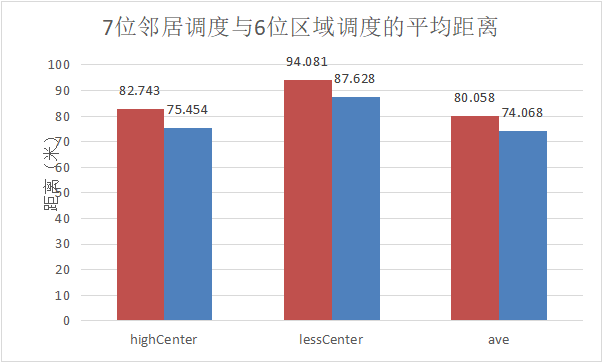
\includegraphics[width=1.0\textwidth]{figures/邻居区域匹配距离}
  \caption{邻居区域匹配距离}\label{fig:regionDistance}
\end{figure}

% \begin{figure}
%   \centering
%   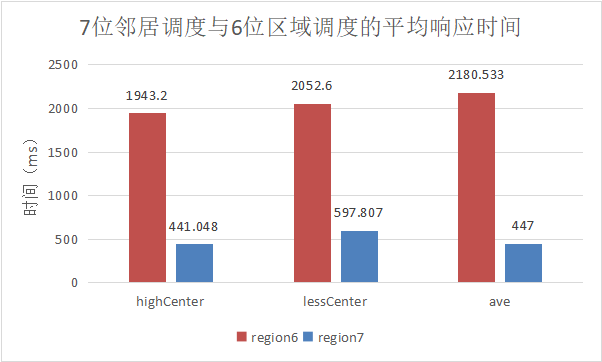
\includegraphics[width=1.0\textwidth]{figures/邻居区域响应时间}
%   \caption{邻居区域响应时间}\label{fig:regionTime}
% \end{figure}
% 高峰和低峰环境下的对比结果(一图)

% 可以观察到,所有乘客进行6位区域调度的响应时间均明显低于全局调度的响应时间。

% 不同位置乘客,其进行全局调度请求的响应时间区别较大。这是因为,查找距离乘客最近的空车时,全局调度需要遍历的车辆较多,若后台未能先找到距离乘客较近的车辆,那么后续找到更近距离的空车后,会多次更改智能合约内部的数据状态,导致响应时间延长。故不同位置的乘客进行全局调度请求时,系统的响应时间区别较大。

% 相比全局调度,相同乘客进行6位区域调度的响应时间低于全局调度的比例为100$\%$,这说明了在出租车调度系统中应用地理位置区块链的正确性和有效性。

% 可以观察到,每个乘客在两种环境下的调度请求结果,有时是全局调度的车辆更远,有时是区域调度的车辆更远,但二者绝大部分的距离结果相差并不大(平均起来,每位乘客与其匹配到的车辆的距离,在6位GeoHash的区域调度时,只比全局调度远$\%$。

% 但值得注意的是,全局调度中会有乘客匹配到明显较远的车辆,其距离是乘客平均等车距离的7.63倍、6.23倍,让少数乘客付出了更多的等待时间。这说明,相比全局调度而言,区域调度能保证匹配到的出租车不会距离乘客太远,从而提高了所有乘客的打车体验,同时还能保持平均调度距离不明显增加。

% 但区域调度显著降低了系统的响应时间,同时保证了所有乘客的打车体验,证明了地理位置区块链的应用相比传统区块链具有明显优势。

% 但基于6位GeoHash的区域调度也有易见的缺点:将可选车辆的范围限制在了6位GeoHash区域的范围内,如果乘客的位置在6位GeoHash区域的边缘,则在该6位区域外的相邻区域可能有比原区域内距离乘客更近的空车。

以乘客位置所在的6位GeoHash区域为中心,根据算法获得其周围的8个邻居区域,地理位置区块链根据这9个区域查询到区域内对应的车辆账户,然后从这些车辆中筛选出距离乘客最近的空车。此调度方法克服单独的6位GeoHash区域调度的边界现象,让车乘匹配的结果更合理。

单独的6位区域调度只能调度到自己所属地理区域内的车辆,当乘客所处的位置位于6位GeoHash地理区域的边缘时,如果这个区域内车辆的数目不够,有部分乘客的打车请求不会被满足,但实际上乘客附近的其它6位GeoHash区域中有空车,而且相距乘客的距离也合适,但因为地理划分的问题没有被考虑。6位邻居区域调度可以根据乘客的位置调度到乘客所处区域和周围邻居区域内最近的空车,减少GeoHash划分的地理区域的限制,能够更好地满足乘客的打车需求。

实验数据表明,6位邻居调度调度结果的车乘平均距离,比单独6位GeoHash区域调度结果的车乘平均距离更近,这是因为邻居区域调度优化了单独区域调度的边界限制,乘客在6位GeoHash地理区域边缘可以匹配到邻居区域内实际距离更近的车辆,而不是匹配到本区域内更远的车辆。



\section{传统区块链与地理位置区块链的系统对比实验}

系统测试实验从实际应用的方面探究本文所提出方法的实用性和正确性。分为模拟道路的系统实验和真实道路的系统实验两部分。

【贾兴无】的工作分析了工作日居民选择出租车出行的供需图,其工作统计出,在高峰时段,乘客的出行需求数目可达同时段空驶出租车供给数目的约1.5倍,在平峰时段,乘客的出行需求数目仅仅略高于空驶出租车的供给数目。贾的工作将城市核心区根据不同的土地性质划分为居住区、商业区等交通小区,交通小区的直径在0.5km到2.5km之间,工作日各交通小区的高峰某时刻的出租车需求频数在20至200之间,高峰期各个交通小区每小时的出租车需求频数在60至600之间,本文的系统测试选取2.5km规模的区域进行调度系统的初始化和运行,观察本文所提出的理论工具的实际效果。

系统首先测试了交通小区内高峰期不同初始化车辆状态时,基于传统区块链的全局调度和基于地理位置区块链的区域调度之间的性能差别。考虑到交通小区的范围在0.5km到2.5km之间,选取一个5位GeoHash地图瓦片覆盖的交通小区,交通小区内的道路采用模拟真实路段数据的双行道,小区内每个6位GeoHash瓦片覆盖4个十字路口。在交通小区内模拟高峰期的打车时刻,乘客的出行数量为空驶出租车供给数量的1.5倍,车辆的位置和乘客的上车点在区域内随机均匀分布。保持高峰时刻车辆和乘客的比例,改变两者的数值,得到高峰时传统区块链环境和地理位置区块链环境下系统运行的响应性能对比图\ref{fig:compare}。

\begin{figure}
  \centering
  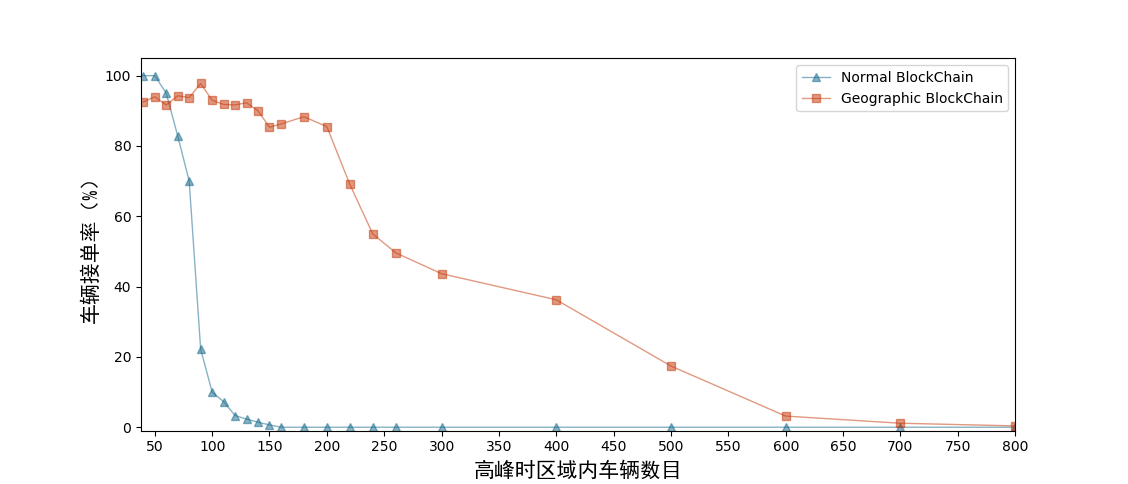
\includegraphics[width=1.0\textwidth]{figures/性能对比}
  \caption{性能对比}\label{fig:compare}
\end{figure}

横轴为高峰期初始时刻交通小区内初始化的车辆数目(乘客需求数量保持为车辆数量的1.5倍),纵轴为高峰期时,乘客发出请求后,交通小区内接到订单的车辆的比率。在传统区块链中,乘客申请调度车辆时,区块链合约维护的车辆信息过多,遍历车辆信息时会发生超时现象,此时乘客呼叫车辆的请求无法得到响应,导致区域内车辆获取不到乘客的打车信息,接单率不理想。上图在区域内初始化车辆数目为50左右时,传统区块链环境下的车辆接单率为100$\%$,此时区域内所有乘客呼叫车辆不会发生超时。当区域内初始化的车辆数目达到160的规模时,传统区块链后台超过负载极限,无法正常响应交通小区内所有的乘客打车请求,区域内的空驶车辆无法接到订单。

​在地理位置区块链做后台的环境下,由于地理位置区块链后台可以直接查询到乘客附近区域内的车辆账户,避免了对全局的大规模车辆账户进行低效的查询,故响应性能相比传统区块链后台有提升。在区域内车辆分布较多时,地理位置区块链支持的系统中,车辆的接单率平均保持在90$\%$及以上的水平。交通小区内车辆分布数为180辆左右时,所有乘客的打车请求均不会超时。此时若乘客所在附近区域内有空车,乘客呼叫车辆的请求均会得到响应。当交通小区内车辆较少时,在地理位置区块链做后台的环境下,由于部分乘客的邻居区域内没有可调度的空车,故在这一时刻的呼车请求没有得到及时的响应,但该交通小区内所有车辆的接单率仍保持在90$\%$以上的水平。当交通小区内的车辆超过200辆后,乘客的打车请求会有一部分超时,地理位置区块链后台不能及时响应部分请求,导致车辆的接单率下降,此后随着小区内车辆和乘客请求密度的增加,地理位置区块链的响应超时的比例也会增加,直到车辆密度达到800时,区块链后台对所有的请求服务均超时,地理位置区块链后台超过负载极限。

在传统区块链与地理位置区块链都能支持的出行规模中,对比两种环境下,出租车调度系统运行后的各项数值。在与上述同样规模的交通小区内模拟高峰期持续30min的出行需求。初始时区域内有50辆空驶出租车和75个乘客打车需求随机均匀分布,其余的空驶车辆和乘客打车需求在30min内均匀加入到调度系统中,系统运行期间总共处理加入100辆出租车和150位乘客订单,系统运行期间收集的数据信息包括:两种后台环境下的车辆载客时间占比图\ref{fig:loadPropotion}、乘客距离接单车辆的距离图\ref{fig:distance}、乘客发出订单到匹配到车辆的响应时间图\ref{fig:manageTime}、区块链后台调度车辆的gas消耗图\ref{fig:gasCost},将收集的数据制作成箱型图进行对比。

\begin{figure}
  \centering
  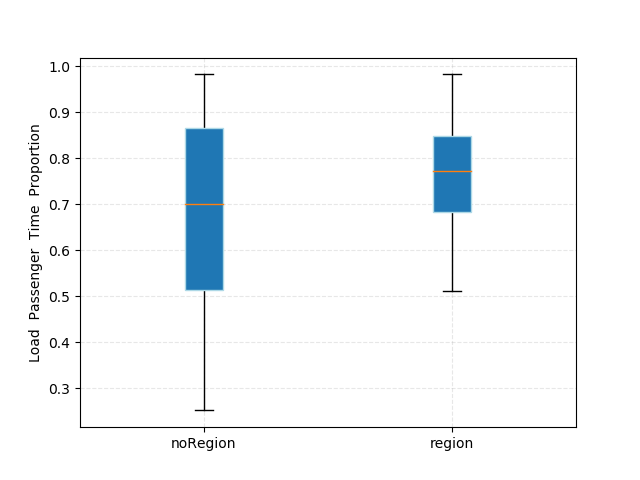
\includegraphics[width=1.0\textwidth]{figures/loadPropotion}
  \caption{车辆载客时间占比}\label{fig:loadPropotion}
\end{figure}

\begin{figure}
  \centering
  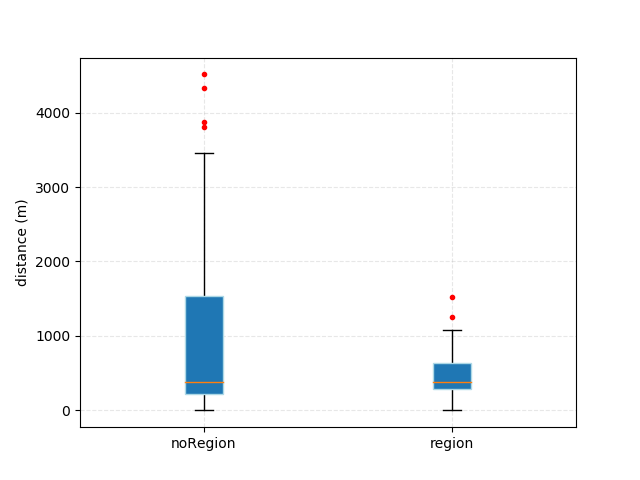
\includegraphics[width=1.0\textwidth]{figures/distance}
  \caption{乘客和接单车辆的距离}\label{fig:distance}
\end{figure}

\begin{figure}
  \centering
  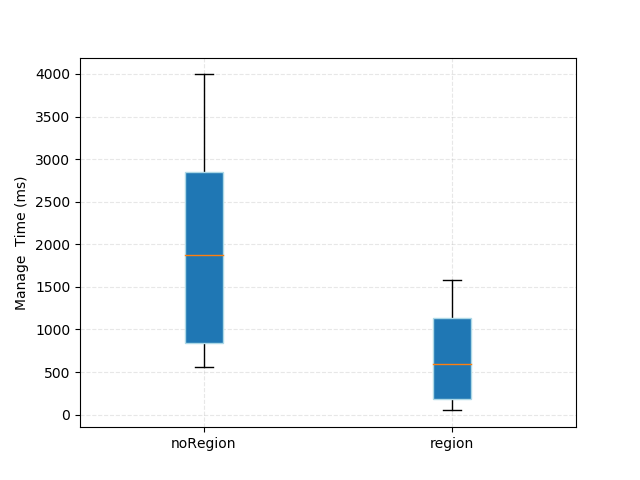
\includegraphics[width=1.0\textwidth]{figures/manageTime}
  \caption{乘客匹配到车辆的响应时间}\label{fig:manageTime}
\end{figure}

\begin{figure}
  \centering
  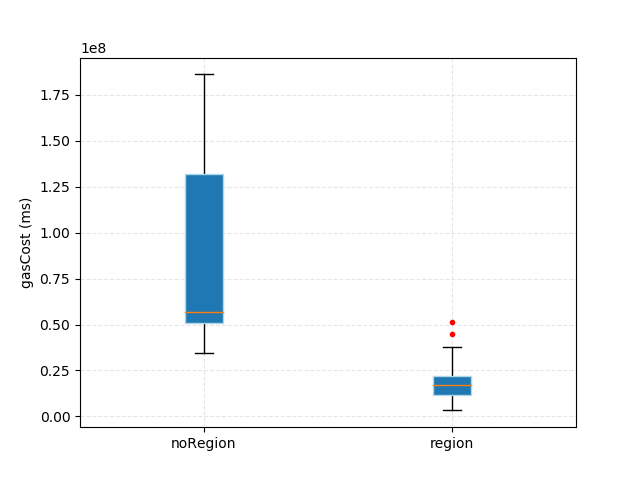
\includegraphics[width=1.0\textwidth]{figures/gasCost}
  \caption{调度车辆的gas消耗}\label{fig:gasCost}
\end{figure}

车辆载客时间占比箱型图\ref{fig:loadPropotion},纵轴为载客时间占车辆订单运行时间的比例,横轴为两种环境下完成订单的同一批车辆个体。从数据统计箱型图可以看到,在地理位置区块链环境下,车辆的载客时间占比更长的情况更多,比传统区块链环境下多$\%$,同时,地理位置区块链区域调度的车辆的载客时间占比分布更集中在0.7及以上,说明在地理位置区块链环境下,大部分出租车的有效载客时间整体得到提高,同一批车辆的载客时间占比中位数,在地理位置区块链环境下比在传统区块链环境下高$\%$,平均值高$\%$,这说明基于地理位置区块链区域调度方法会优化交通小区内车辆的运营效率。

车乘距离箱型图\ref{fig:distance},反映了车辆在接单时与乘客的距离,从图中分析可知,两种环境下,基于地理位置区块链的区域调度的车乘距离的中位数与传统区块链相近,差距仅为$\%$,但区域调度的环境下,车辆与乘客的距离数值分布在较小的范围内,90$\%$以上的接单车辆分布在与乘客距离1000米以内,在传统区块链环境中,,乘车距离的分布更为离散,有一部分接单的车辆相距乘客的距离达到了3000米以上,这明显降低了一部分乘客的打车体验。相比之下,区域调度可以更有效地在合理的区域范围内调度到距离乘客更近的车辆,平均距离减少了$\%$,让区域内乘客等车的时间减少,提高乘客的打车体验。

乘客打车响应时间箱型图\ref{fig:manageTime},反映了乘客发出订单后,到接受服务端返回的匹配到的车辆信息的时间间隔。由图可知,全局调度环境下的打车响应时间相较于区域调度环境下更加离散,区域调度在打车响应时间的指标上具有明显的优势,区域调度车辆的响应时间中位数在600ms左右,全局调度车辆的响应时间中位数在1800ms左右。同时,全局调度中还有部分乘客的响应时间接近4000ms,这是由于全局调度考虑的车辆数目较多,后台修改记录状态的开销增加,导致响应时间增加。在后台运算的gas消耗上,区域调度进行车乘匹配的运算消耗平均是全局调度gas消耗的30$\%$。

\section{系统测试实验}
\subsection{地理位置区块链性能测试实验}
本部分旨在测试地理位置区块链能在多大区域内维护多少个车辆和乘客请求,在4km * 5km的范围内,地理位置区块链能支持200车辆和300乘客的交互规模。可以满足大部分交通小区高峰期的打车规模。
% 区域规模、请求规模,探究不同区域下可以请求多大的规模。探究更大范围的地理区域可以支持多大规模的车乘交互请求,

\begin{figure}
  \centering
  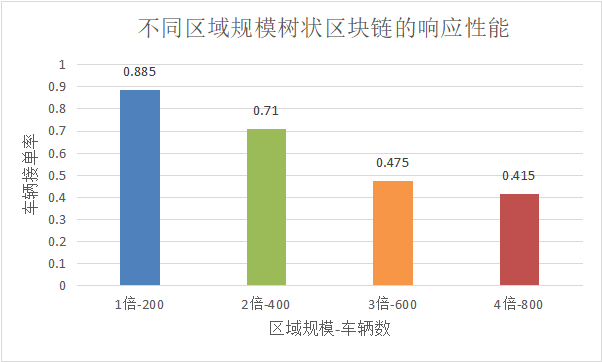
\includegraphics[width=1.0\textwidth]{figures/treeBlockchcainPerformance}
  \caption{树状区块链性能实验}\label{fig:treeBlockchcainPerformance}
\end{figure}

探究地理位置区块链的性能实验,可以通过实验观察基于地理位置区块链的出租车调度系统可以在不同范围区域内满足不同的请求规模,根据其服务特点,可以在不同类型小区的不同时期维护不同规模的节点,从而节省计算资源。

如图\ref{fig:treeBlockchcainPerformance},在1倍区域的规模时,乘客的邻居范围内有空闲车辆时,乘客的打车请求均会得到满足。在2倍区域的规模时,服务端接收到的请求规模翻倍,部分乘客的打车请求会响应超时,车辆的接单率也会因此降低。当区域的规模继续扩大到3倍、4倍时,服务器超时的处理会增多,车辆的接单率降低。

\subsection{系统在模拟道路上的运行实验}
在4km * 5km的区域范围内,初始化200车和300乘客,模拟2小时的高峰期出行环境,2小时共运行800车和1200乘客。
运行结果数据统计如图\ref{fig:2hDistance}和图\ref{fig:2hTime}。2小时内,呼叫到出租车的乘客,其距离车辆的距离最大为1750m左右,80$\%$以上的车辆与乘客的距离在200m-1200m的范围内,乘客调度出租车的合理距离范围。2h系统中,乘客呼叫出租车的响应时间,绝大部分在4s以内,最大响应时间不超过12s。

\begin{figure}
  \centering
  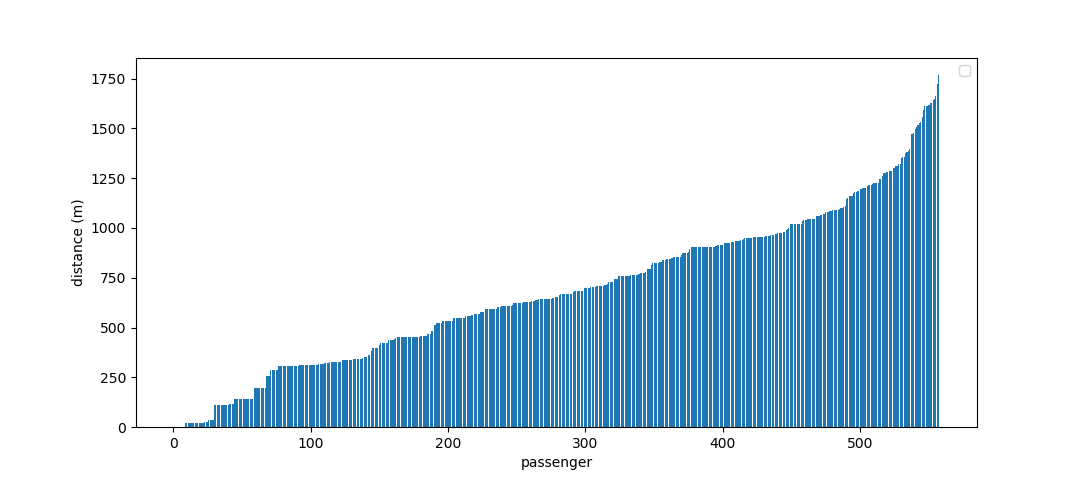
\includegraphics[width=1.0\textwidth]{figures/2hDistance}
  \caption{2小时模拟车乘距离}\label{fig:2hDistance}
\end{figure}

\begin{figure}
  \centering
  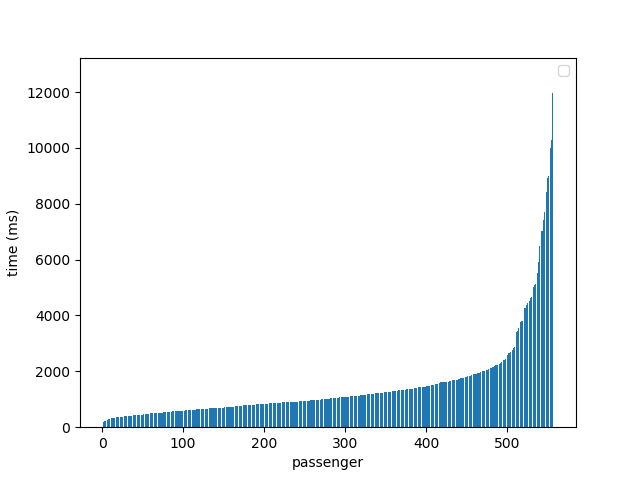
\includegraphics[width=1.0\textwidth]{figures/2hTime}
  \caption{2小时模拟响应时间}\label{fig:2hTime}
\end{figure}

(待补充实验)测试大范围地图区域下系统的特征。初始化车辆和乘客,模拟2小时的出行环境,收集系统运行数据。分析数据可知地理位置区块链服务器在大面积范围内进行系统运行时,乘客呼车的响应时间、车辆与乘客的距离、车辆的载客效率均保持在合理范围内,证明了基于地理位置区块链的系统的健壮性。

\subsection{系统在真实道路上的运行实验}
(待补充实验)在真实地图数据中运行调度系统,收集数据分析可知。基于地理位置区块链的系统比传统区块链的系统,车辆的平均载客时间更长,乘客打车的响应时间更短,匹配到的车辆相距乘客的距离更近。真实地图数据的实验更能说明应用地理位置区块链进行区域调度的优越性,在真实场景中得到了验证。

% \begin{figure}
%   \centering
%   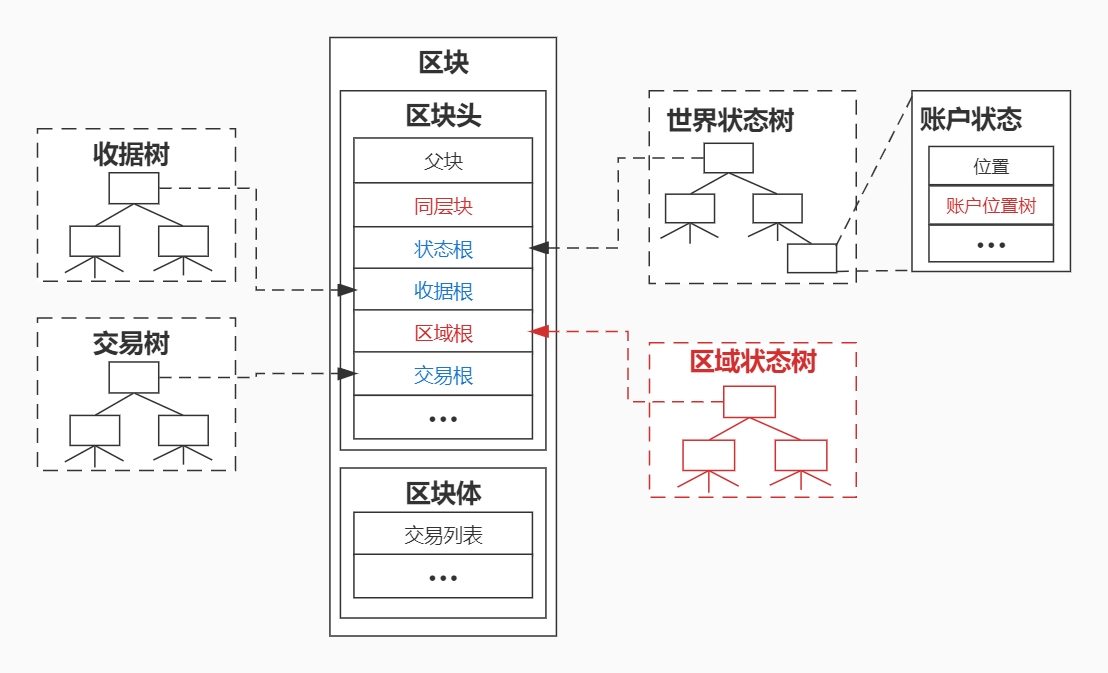
\includegraphics[width=1.0\textwidth]{figures/树状区块链}
%   \caption{树状区块链数据结构变化图}\label{fig:treeBlockchain}
% \end{figure}

(待补充实验)在真实地图数据中测试地理位置区块链的性能,分析交通小区的运行结果可知。本文所提出系统在实际地图的运行中,其收集到的结果包括乘客打车响应时间、车辆相距乘客的距离、车辆的载客时间占比等均处在合理的范围内。说明本出租车调度系统可以在真实的地图数据中正常运行并得到合理的结果。本工作将地理信息与区块链相结合,简化了计算方式,优化了计算效率,并且可以基于地理信息设计有效的方法来研发应用,有效验证了结合地理信息的区块链在车载自组网方向上的实用性。

% \begin{figure}
%   \centering
%   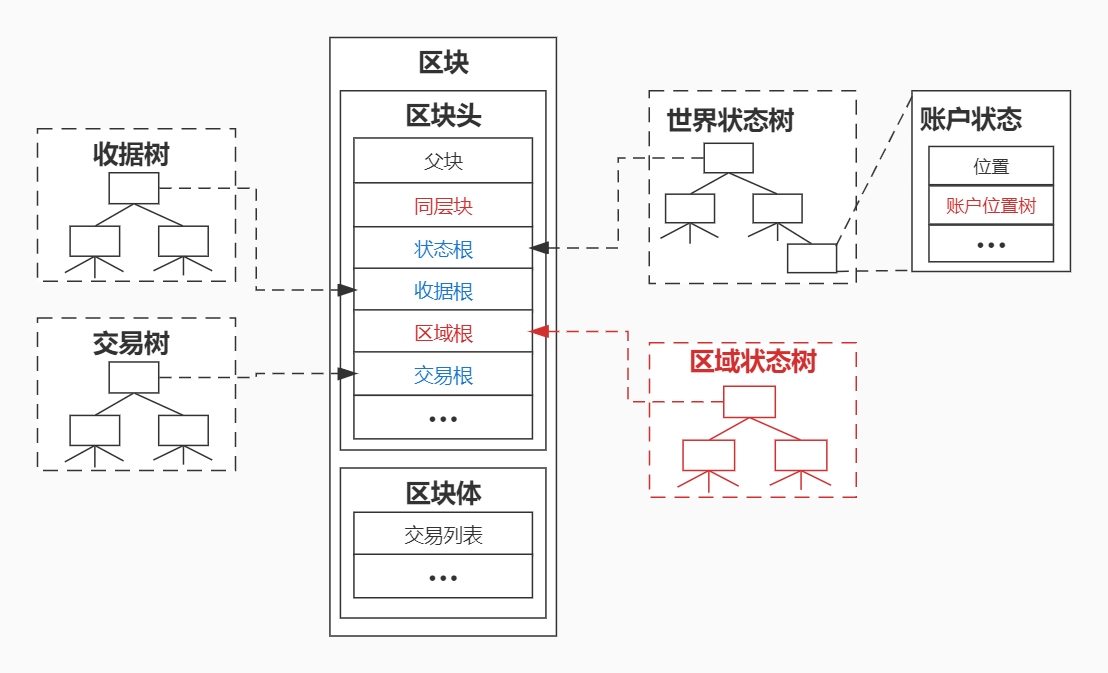
\includegraphics[width=1.0\textwidth]{figures/树状区块链}
%   \caption{树状区块链数据结构变化图}\label{fig:treeBlockchain}
% \end{figure}

% \section{数据分析工作}

% 1. 出租车GPS数据字段包括是否载客的状态,利用对出租车是否载客的分析可以得到出租车的分布特点和乘客的分布特点。

% 2. 分析真实的出租车数据,讨论不同时段的车辆和乘客在城区的分布情况(既考虑了时间因素也考虑了位置因素),依此设置空车和乘客的初始化位置和比例,为下一步系统仿真测试做铺垫。

% \section{系统测试实验}

% 展示近距离路径规划和远距离路径规划的路径

% \subsection{真实地图数据测试}
% 真实地图的路径规划结果测试。

% 收集数据:
% 1. 在不同环境下(请求频繁或者稀疏)乘客平均等待时间、车辆平均空车时间(即处于未载客状态的时间),或者百分率,验证区域调度相比全局调度的优越性,系统将区块链与地理信息结合是有意义的。
% 2. 在不同环境下(请求频繁或者稀疏)系统对乘客请求的响应时间,响应时间在一定阈值范围内,可验证系统的合理性和正确性。